% SpatialMoE-SOD architecture overview (Fig. 1)
% Canvas is exactly 153 mm wide (= \textwidth of the manuscript), so include it at
% width=\textwidth and every label prints at its true size (6 pt body text).
% Optional thumbnails: figs/input.png, figs/gt.png, figs/saliency.png, figs/boundary.png.
% If a file is missing a neutral drawn placeholder is used, so this always compiles.
\documentclass[tikz,border=0pt]{standalone}
\usepackage[T1]{fontenc}
\usepackage{helvet}
\renewcommand{\familydefault}{\sfdefault}
\usepackage{amsmath,amssymb}
\usepackage{sansmath}
\usepackage{graphicx}
\usetikzlibrary{arrows.meta,calc}

% ---------------------------------------------------------------- palette
\definecolor{bbF}{HTML}{DCE8F5}  \definecolor{bbS}{HTML}{4F76A3}
\definecolor{moF}{HTML}{FBEFC2}  \definecolor{moS}{HTML}{B08D2B}  \definecolor{moD}{HTML}{E9CF74}
\definecolor{enF}{HTML}{F8DCC8}  \definecolor{enS}{HTML}{C07A3E}
\definecolor{dcF}{HTML}{DCEBD2}  \definecolor{dcS}{HTML}{6B8F4E}
\definecolor{hdF}{HTML}{E4DDF0}  \definecolor{hdS}{HTML}{7D6AA3}
\definecolor{ink}{HTML}{333333}  \definecolor{sup}{HTML}{777777}

% ---------------------------------------------------------------- styles
\tikzset{
  base/.style={font=\sansmath\sffamily\fontsize{6}{7}\selectfont, align=center, text=black},
  big/.style={font=\sansmath\sffamily\fontsize{6.5}{7.5}\selectfont\bfseries},
  box/.style={base, draw, line width=0.5pt, rounded corners=1.5pt, inner sep=1.5pt},
  flow/.style={-{Stealth[length=1.5mm,width=1.2mm]}, line width=0.6pt, draw=ink, rounded corners=2pt},
  conf/.style={flow, draw=enS, dash pattern=on 2pt off 1.5pt},
  supv/.style={flow, draw=sup, dash pattern=on 2pt off 1.5pt},
  plain/.style={line width=0.6pt, draw=ink},
  plus/.style={draw=enS, fill=enF, line width=0.5pt},
}

% ---------------------------------------------------------------- thumbnails
% \thumbmask{file}{cx}{cy}{size}{kind}   kind: 0 = filled mask, 1 = outline (boundary)
\newcommand{\thumbmask}[5]{%
  \IfFileExists{#1}%
  {\node[inner sep=0, draw=black!60, line width=0.4pt] at (#2,#3)
     {\includegraphics[width=#4 cm,height=#4 cm]{#1}};}%
  {\fill[black] (#2-#4/2,#3-#4/2) rectangle (#2+#4/2,#3+#4/2);
   \ifnum#5=0
     \fill[white] (#2,#3) ellipse ({#4*0.30} and {#4*0.24});
   \else
     \draw[white, line width=0.5pt] (#2,#3) ellipse ({#4*0.30} and {#4*0.24});
   \fi
   \draw[black!60, line width=0.4pt] (#2-#4/2,#3-#4/2) rectangle (#2+#4/2,#3+#4/2);}}
\newcommand{\thumbinput}[4]{%
  \IfFileExists{#1}%
  {\node[inner sep=0, draw=black!60, line width=0.4pt] at (#2,#3)
     {\includegraphics[width=#4 cm,height=#4 cm]{#1}};}%
  {\fill[black!12] (#2-#4/2,#3-#4/2) rectangle (#2+#4/2,#3+#4/2);
   \fill[black!38] (#2,#3-#4*0.04) ellipse ({#4*0.28} and {#4*0.22});
   \draw[black!60, line width=0.4pt] (#2-#4/2,#3-#4/2) rectangle (#2+#4/2,#3+#4/2);}}

\begin{document}
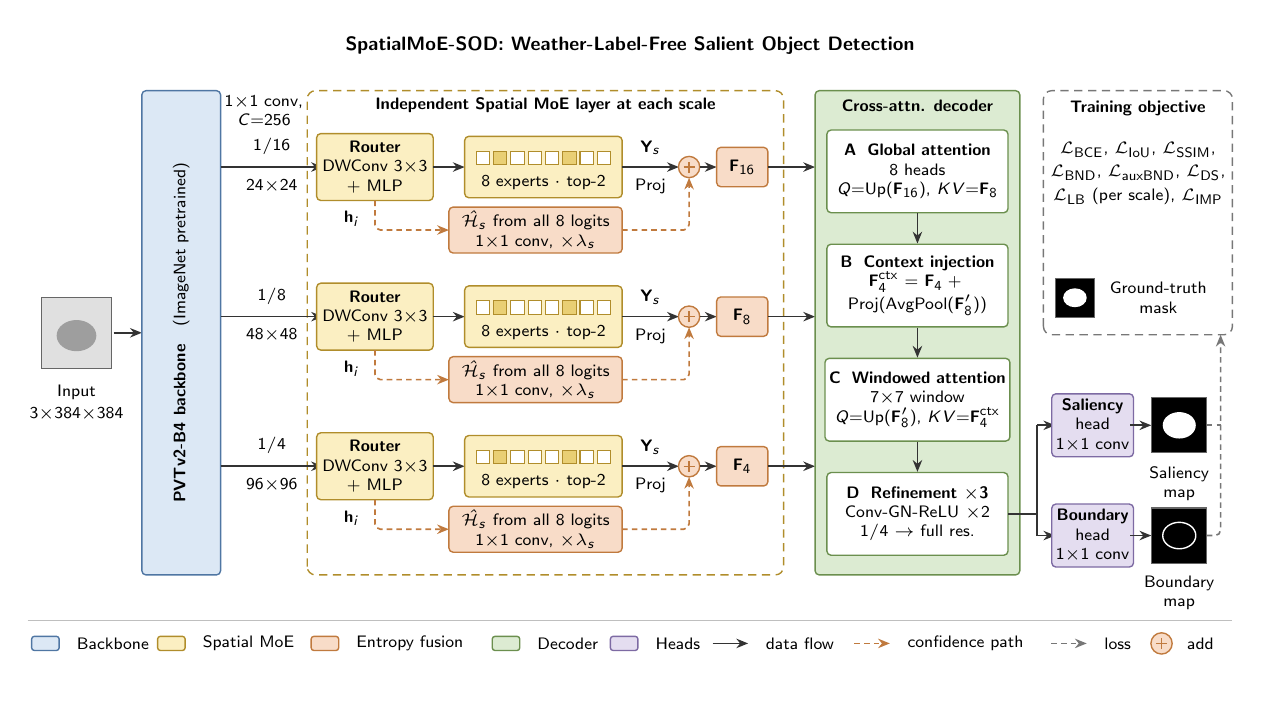
\begin{tikzpicture}[x=1cm,y=1cm]
% fixed canvas: 153 mm x 82 mm
\useasboundingbox (0,-0.15) rectangle (15.3,8.05);

% ------------------------------------------------------------------ title
\node[font=\sansmath\sffamily\fontsize{7.5}{8.5}\selectfont\bfseries] at (7.65,7.82)
  {SpatialMoE-SOD: Weather-Label-Free Salient Object Detection};

% ------------------------------------------------------------------ input
\thumbinput{figs/input.png}{0.62}{4.175}{0.9}
\node[base, anchor=north] at (0.62,3.64) {Input\\[1pt]$3{\times}384{\times}384$};
\draw[flow] (1.09,4.175) -- (1.45,4.175);

% ------------------------------------------------------------------ backbone
\draw[draw=bbS, fill=bbF, line width=0.5pt, rounded corners=1.5pt] (1.45,1.1) rectangle (2.45,7.25);
\node[base, rotate=90] at (1.95,4.175)
  {{\bfseries PVTv2-B4 backbone}\quad(ImageNet pretrained)};
\node[base] at (3.0,7.0) {1$\times$1 conv,\\$C{=}256$};

% ------------------------------------------------------------------ Spatial MoE group
\draw[draw=moS, dash pattern=on 3pt off 2pt, line width=0.5pt, rounded corners=3pt] (3.55,1.1) rectangle (9.6,7.25);
\node[base, font=\sansmath\sffamily\fontsize{6.5}{7.5}\selectfont\bfseries] at (6.575,7.06)
  {Independent Spatial MoE layer at each scale};

% rows: scale / spatial size / row centre
\foreach \s/\hw/\yc in {16/24/6.0, 8/48/4.1, 4/96/2.2}{
  \pgfmathsetmacro{\ym}{\yc+0.28}
  \pgfmathsetmacro{\ye}{\yc-0.52}
  % backbone -> router
  \draw[flow] (2.45,\ym) -- (3.75,\ym);
  \node[base, anchor=south] at (3.1,\ym+0.03) {$1/\s$};
  \node[base, anchor=north] at (3.1,\ym-0.03) {$\hw{\times}\hw$};
  % router
  \node[box, draw=moS, fill=moF, minimum width=1.48cm, minimum height=0.85cm] (R\s) at (4.41,\ym)
    {{\bfseries Router}\\DWConv 3$\times$3\\$+$ MLP};
  \draw[flow] (5.15,\ym) -- (5.55,\ym);
  % experts
  \node[box, draw=moS, fill=moF, minimum width=2.0cm, minimum height=0.78cm] (X\s) at (6.55,\ym) {};
  \foreach \e in {0,...,7}{
    \pgfmathsetmacro{\ex}{5.695+\e*0.22}
    \ifnum\e=1 \def\efill{moD}\else\ifnum\e=5 \def\efill{moD}\else\def\efill{white}\fi\fi
    \draw[draw=moS, fill=\efill, line width=0.4pt] (\ex,\ym+0.03) rectangle (\ex+0.17,\ym+0.2);
  }
  \node[base] at (6.55,\ym-0.2) {8 experts $\cdot$ top-2};
  % experts -> plus
  \draw[flow] (7.55,\ym) -- (8.27,\ym);
  \node[base, anchor=south] at (7.91,\ym+0.03) {$\mathbf{Y}_s$};
  \node[base, anchor=north] at (7.91,\ym-0.03) {Proj};
  \node[circle, plus, inner sep=0, minimum size=0.27cm] (P\s) at (8.4,\ym) {};
  \draw[enS, line width=0.5pt] (8.4-0.07,\ym) -- (8.4+0.07,\ym) (8.4,\ym-0.07) -- (8.4,\ym+0.07);
  \draw[flow] (8.535,\ym) -- (8.75,\ym);
  \node[box, draw=enS, fill=enF, minimum width=0.65cm, minimum height=0.5cm] (F\s) at (9.075,\ym)
    {$\mathbf{F}_{\s}$};
  % entropy branch (from the full 8-way logits)
  \node[box, draw=enS, fill=enF, minimum width=2.2cm, minimum height=0.46cm] (H\s) at (6.45,\ye)
    {$\hat{\mathcal{H}}_s$ from all 8 logits\\1$\times$1 conv, $\times\lambda_s$};
  \draw[conf] (4.41,\ym-0.425) -- (4.41,\ye) -- (5.35,\ye);
  \node[base, anchor=east] at (4.34,\ye+0.14) {$\mathbf{h}_i$};
  \draw[conf] (7.55,\ye) -- (8.4,\ye) -- (8.4,\ym-0.135);
  % F -> decoder
  \draw[flow] (9.4,\ym) -- (10.0,\ym);
}

% ------------------------------------------------------------------ decoder
\draw[draw=dcS, fill=dcF, line width=0.5pt, rounded corners=1.5pt] (10.0,1.1) rectangle (12.6,7.25);
\node[base, font=\sansmath\sffamily\fontsize{6.5}{7.5}\selectfont\bfseries] at (11.3,7.06) {Cross-attn. decoder};
\node[box, draw=dcS, fill=white, minimum width=2.3cm, minimum height=1.05cm] (DA) at (11.3,6.225)
  {{\bfseries A\; Global attention}\\8 heads\\$Q{=}\mathrm{Up}(\mathbf{F}_{16})$, $KV{=}\mathbf{F}_8$};
\node[box, draw=dcS, fill=white, minimum width=2.3cm, minimum height=1.05cm] (DB) at (11.3,4.775)
  {{\bfseries B\; Context injection}\\$\mathbf{F}_4^{\mathrm{ctx}}=\mathbf{F}_4+{}$\\$\mathrm{Proj}(\mathrm{AvgPool}(\mathbf{F}'_8))$};
\node[box, draw=dcS, fill=white, minimum width=2.3cm, minimum height=1.05cm] (DC) at (11.3,3.325)
  {{\bfseries C\; Windowed attention}\\$7{\times}7$ window\\$Q{=}\mathrm{Up}(\mathbf{F}'_8)$, $KV{=}\mathbf{F}_4^{\mathrm{ctx}}$};
\node[box, draw=dcS, fill=white, minimum width=2.3cm, minimum height=1.05cm] (DD) at (11.3,1.875)
  {{\bfseries D\; Refinement $\times$3}\\Conv-GN-ReLU $\times$2\\$1/4\to$ full res.};
\draw[flow] (DA.south) -- (DB.north);
\draw[flow] (DB.south) -- (DC.north);
\draw[flow] (DC.south) -- (DD.north);

% ------------------------------------------------------------------ heads and outputs
\draw[plain] (12.45,1.875) -- (12.82,1.875);
\draw[plain] (12.82,1.6) -- (12.82,3.0);
\draw[flow] (12.82,3.0) -- (13.05,3.0);
\draw[flow] (12.82,1.6) -- (13.05,1.6);
\node[box, draw=hdS, fill=hdF, minimum width=0.95cm, minimum height=0.8cm] (HS) at (13.525,3.0)
  {{\bfseries Saliency}\\head\\1$\times$1 conv};
\node[box, draw=hdS, fill=hdF, minimum width=0.95cm, minimum height=0.8cm] (HB) at (13.525,1.6)
  {{\bfseries Boundary}\\head\\1$\times$1 conv};
\draw[flow] (14.0,3.0) -- (14.27,3.0);
\draw[flow] (14.0,1.6) -- (14.27,1.6);
\thumbmask{figs/saliency.png}{14.625}{3.0}{0.7}{0}
\thumbmask{figs/boundary.png}{14.625}{1.6}{0.7}{1}
\node[base, anchor=north] at (14.625,2.6) {Saliency\\map};
\node[base, anchor=north] at (14.625,1.21) {Boundary\\map};

% ------------------------------------------------------------------ training objective
\draw[draw=sup, dash pattern=on 3pt off 2pt, line width=0.5pt, rounded corners=3pt] (12.9,4.15) rectangle (15.3,7.25);
\node[base, font=\sansmath\sffamily\fontsize{6.5}{7.5}\selectfont\bfseries] at (14.1,7.03) {Training objective};
\node[base] at (14.1,6.2)
  {$\mathcal{L}_{\mathrm{BCE}}$, $\mathcal{L}_{\mathrm{IoU}}$, $\mathcal{L}_{\mathrm{SSIM}}$,\\[1.5pt]
   $\mathcal{L}_{\mathrm{BND}}$, $\mathcal{L}_{\mathrm{auxBND}}$, $\mathcal{L}_{\mathrm{DS}}$,\\[1.5pt]
   $\mathcal{L}_{\mathrm{LB}}$ (per scale), $\mathcal{L}_{\mathrm{IMP}}$};
\node[base, anchor=west] at (13.62,4.62) {Ground-truth\\mask};
\thumbmask{figs/gt.png}{13.3}{4.62}{0.5}{0}
\draw[supv] (14.975,1.6) -- (15.15,1.6) -- (15.15,4.15);
\draw[plain, draw=sup, dash pattern=on 2pt off 1.5pt] (14.975,3.0) -- (15.15,3.0);

% ------------------------------------------------------------------ legend
\draw[draw=black!25, line width=0.3pt] (0,0.52) -- (15.3,0.52);
\newcommand{\lgsw}[3]{\draw[draw=#2, fill=#1, line width=0.5pt, rounded corners=1pt] (#3,0.14) rectangle (#3+0.35,0.32);}
\lgsw{bbF}{bbS}{0.05}   \node[base, anchor=west] at (0.5,0.23)  {Backbone};
\lgsw{moF}{moS}{1.65}   \node[base, anchor=west] at (2.1,0.23)  {Spatial MoE};
\lgsw{enF}{enS}{3.6}    \node[base, anchor=west] at (4.05,0.23) {Entropy fusion};
\lgsw{dcF}{dcS}{5.9}    \node[base, anchor=west] at (6.35,0.23) {Decoder};
\lgsw{hdF}{hdS}{7.4}    \node[base, anchor=west] at (7.85,0.23) {Heads};
\draw[flow] (8.7,0.23) -- (9.15,0.23);     \node[base, anchor=west] at (9.25,0.23)  {data flow};
\draw[conf] (10.5,0.23) -- (10.95,0.23);   \node[base, anchor=west] at (11.05,0.23) {confidence path};
\draw[supv] (13.0,0.23) -- (13.45,0.23);   \node[base, anchor=west] at (13.55,0.23) {loss};
\node[circle, plus, inner sep=0, minimum size=0.27cm] at (14.4,0.23) {};
\draw[enS, line width=0.5pt] (14.33,0.23) -- (14.47,0.23) (14.4,0.16) -- (14.4,0.30);
\node[base, anchor=west] at (14.6,0.23) {add};
\end{tikzpicture}
\end{document}
